\section{Data preprocessing}
\label{section:Data:Preprocessing}
This section briefly describes all the data processing done.

\subsection{Feature Ingeneering}
Both the feature \textit{"hits"} and \textit{"clicks"} can be argued to measure
user interest. A products hits score measure how many times someone has clicked
on to that product information page at prisuigen.no. A products click score measure
how many times prisguiden.no has redirected an user to an external retailer for the given product.
We ended up combining these two variables into one feature which we called \textbf{"interest"}
with the equation defined in \Cref{eq:interest}.
\begin{equation}
  interest = hits + clicks
  \label{eq:interest}
\end{equation}

\subsection{Value Scaling}
For the neural net models we scale using normalization for the ranges to be in the range [0.1, 1].
The unconventional choise of having 0.1 as our lower bound is becuase the matric SMAPE
is vulnerable to zero values, as described in \Cref{eq:sMape}.
Normization was chosen over standardization because we do not know the distrubtion
of the data, and we did not want to assume it followed a Gaussion distribution.
All model output and predictions are rescaled to it's original range before
visualizing and plotting.

For the ARIMA models we did not scale the data because ARIMA models will not
get the same benefits by scaling the input data.

%The way our data pipeline was constructued made it self documenting,
%which means it prints out all the processing steps and saves them as the
%experiment is conducted. This section will briefly cover how the data was processed
%before each type of experiments.
%The different model structures required some differences in processing steps.

\subsection{Univariate to Multivariate feature engeneering}
Since the E-commerce domain is heavily influenced by external factors, such as
holidays, Christmas, and yearly seasons we thought it would be beneficial
for the neural net models to be aware of which day of the week it is,
which month it is, and if it is closer to summer than winter.

We add the \textit{month} feature, a number between [0, 11] depending on which month.

We add the \textit{day} feature, a number between [0, 6] where 6 is saturday, 0 is sunday etc.
We can calculate the day of the week using the formula \Cref{eq:day_of_the_week}
from \Cref{section:BT:day-of-the-week-formula}.

We add the feature \textit{season} which is a number between [-1, 1] using \Cref{eq:season_feature}.

\begin{equation}
  season = \cos(\pi * (month \mod{12}) / 6)
  \label{eq:season_feature}
\end{equation}

\begin{figure}[h!]
  \centering
  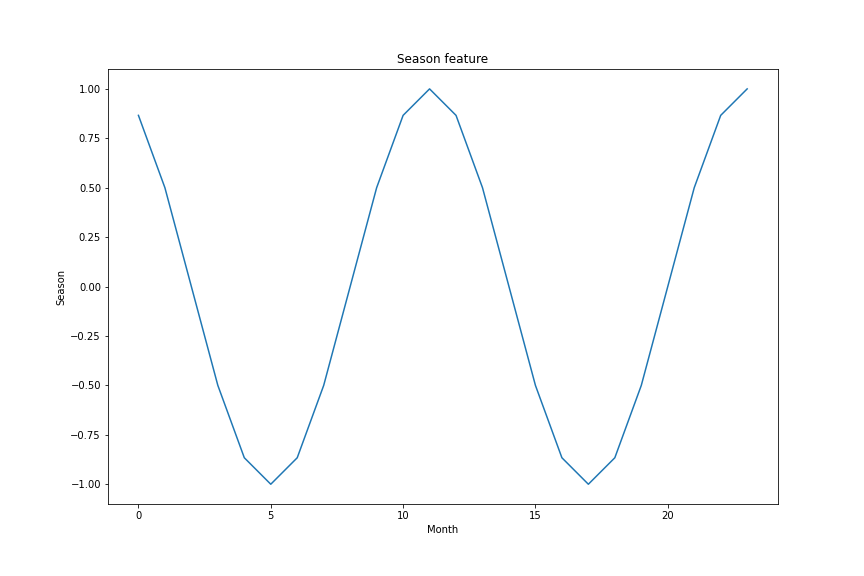
\includegraphics[width=\textwidth]{./figs/code_generated/season_feature.png}
  \hfill
  \caption{Season feature}
  \label{fig:season-feature}
\end{figure}

\Cref{fig:season-feature} shows the output of the season feature.
If the month is close to Christmas (december, januar) this feature will be close to 1.
If the month is closer to summer (may, june) this feature will be close to -1.

In the and all added features are scaled between [0.1, 1] as described above.

\subsubsection{Moving Window Approach}
We are using the same approach  as in \cite{Bandara2019} %Sales Demband FOrecast in E-commerce
and \cite{Hewamalage2021}% Current state and future predictions
\todo[inline]{Write this section.}
\begin{figure}[h!]
  \centering
  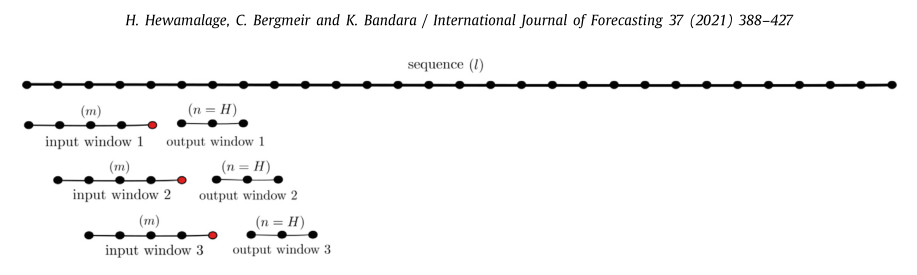
\includegraphics[width=\textwidth]{./figs/illustrations/moving_window_illustration.png}
  \hfill
  \caption{Moving window scheme \citep{Hewamalage2021}}
  \label{fig:dataset:moving_window_scheme}
\end{figure}

\subsection{Train, validation, test splitting}
% The training and validation datasets were seperated in a manner similar
% to that described by \cite{Bandara2019} and \cite[]{Hewamalage2021}.

The inspiration of the trainining, validation and test splitting is taken from
\cite{Bandara2019}, \cite{Hewamalage2021}.
Both reserves the last $m$ sized part for validation from the training data,
where $m$ is the forecasting window size.
% This means L - 2*(n+ m)
%\cite{Hewamalage2021} reserves the last $m$ sized part for validation,
%where $m$ is the forecasting window size.
But \cite{Hewamalage2021} they point out that this is problematic becouse the last part of the sequence is
not considered for training the model.
The further away the test predictions are from the training set the worse,
because the underlying patterns may change during this last part of the sequence.
Therefore \cite{Hewamalage2021} will split the dataset during tuning, but when testing
they will train on all the available training data.

We made some modifications of \cite{Hewamalage2021} data split solution.
First, we have the complete datasets available, so we had to split out our
test set manually. Our test set from each time series consist of the last $m$ sized
sequence for forecasting.

Second, we used a stateful LSTM, which restricted the validation set to have the
same batch size as the training set. This meant that having a validation set equal
to the size of the forecast window $m$ would limit the batch size of the training set
to use a batch size equal to $m$. \cite{Bandara2019} would always
train their models on multiple time series, which meant that their validation set would
be $validation\_size = m * number\_of\_series$. In contrast we would also train models on
a single time series. In this case the validation set would be equal to one forecasting window.
When the forecasting window was of size 7 we found that this validation set got too small.
We experienced a wide range of optimal hyperparameters. These models did not seem to
learn anything meaninfule patterns from the training data, but would in most cases guess
the median.

As a result of the findings above we chose a batch size for the training set first, then
used the chosen batch size as a validation size.
This solution means that we cannot do a hyperparameter search for an optimal batch size
because that would change the validation set as well. When we tried this, the model would
almost always prefere the smallest possible batch size because that meant it would get a
small validation set, which also meant fewer possible errors it could make.

Same as \cite[]{Hewamalage2021} we would also split the training set into validation set for
hyperparameter tuning, but for testing we would train on the validation set as well.

%part L - (IW + OW) as test set,
%and the next part for validation L - 2(IW + OW) during tuning.
%But for testing and prediction they will train on the validation set as well
%because the last part of the sequence is not considered for training the model.
%The further away the test predictions are frin the training set, the worse
%because the underlying patterns may change during this last part of the sequence.


\begin{figure}[h!]
  \centering
  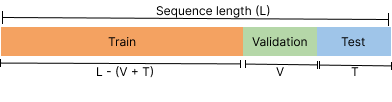
\includegraphics[width=0.7\textwidth]{./figs/illustrations/illustration_train_val_test_split.png}
  \hfill
  \caption{Illustration of trainig, validation, and test split. V = batch size, T = m = forecast window}
  \label{fig:train-val-test-split}
\end{figure}

\Cref{fig:train-val-test-split} shows an illustration of how one dataset is split up during
hyperparameter tuning.
The whole time series has a size of length $L$. The test set $T$ is taken from the end of the series,
and has the size of the forecast window $L = m$. The validation set $V$ has the size of
one batch size $V=batch\_size$. So during tuning the size of the training data is
$T = L - (V + T)$. During testing the validation set $V$ is re-added to the training set,
making the training set $T = L - T$.

\begin{figure}[h!]
  \centering
  
\includegraphics[width=0.7\textwidth]{./figs/illustrations/illustration_global_time_series.png}
  \hfill
  \caption{Illustration of how multiple time series are concatonated for the global method}
  \label{fig:global-time-series}
\end{figure}